\documentclass[12pt,a4paper]{article}

% --------------------------------------------------
% Paquetes
% --------------------------------------------------

% Símbolos y matemáticas
\usepackage{fdsymbol}
\usepackage{amsmath}
\usepackage{amssymb}
\usepackage{amsthm}

% Algoritmos
\usepackage{algpseudocode}

% Tablas y columnas
\usepackage{multirow}
\usepackage{multicol}

% Imágenes y comentarios
\usepackage{graphicx}
\usepackage{float}
\usepackage{comment}

% Código fuente
\usepackage{listings}
\usepackage{xcolor}

% Configuración de idioma
\usepackage[utf8]{inputenc}
\usepackage[T1]{fontenc}
\usepackage[spanish,es-nodecimaldot]{babel}

% Enumeraciones
\usepackage{enumitem}

% Márgenes
\usepackage[
    top=3cm,
    bottom=3cm,
    left=2cm,
    right=2cm,
    heightrounded
]{geometry}

% Hipervínculos
\usepackage{hyperref}

% --------------------------------------------------
% Configuración de código
% --------------------------------------------------

\definecolor{codegray}{gray}{0.95}
\definecolor{dkgreen}{rgb}{0,0.45,0}

\lstset{
    backgroundcolor=\color{codegray},
    basicstyle=\ttfamily\small,
    frame=single,
    breaklines=true,
    columns=fullflexible,
    keepspaces=true,
    showstringspaces=false
}

% --------------------------------------------------
% Encabezado y pie de página
% --------------------------------------------------

\usepackage{fancyhdr}

\pagestyle{fancy}
\fancyhf{}

\cfoot{\thepage}
\lhead{Tarea 2}
\rhead{\textsc{Cómputo Concurrente}}

% --------------------------------------------------
% Documento
% --------------------------------------------------

\begin{document}

\begin{titlepage}
    \thispagestyle{empty}
    \begin{minipage}[c][0.17\textheight][c]{0.25\textwidth}
        \begin{center}
            
\includegraphics[width=3.5cm, height=3.5cm]{Imagenes/LogoUNAM.png}
        \end{center}
    \end{minipage}
    \begin{minipage}[c][0.195\textheight][t]{0.75\textwidth}
        \begin{center}
            \vspace{0.3cm}
            \hrule height2.5pt
            \vspace{.2cm}
            \hrule height1pt
            \vspace{2.0cm}
            \textsc{\Large Universidad Nacional Autónoma de México}\\[1cm]
            \textsc{\Large Facultad de Ciencias}\\[0.5cm]
        \end{center}
    \end{minipage}
    
    \begin{minipage}[c][0.81\textheight][t]{0.25\textwidth}
        \vspace*{5mm}
        \begin{center}
            \hskip2.0mm
            \vrule width1pt height13cm 
            \hskip2pt
            \vrule width2.5pt height13cm
            \hskip2mm
            \vrule width1pt height13cm \\
            \vspace{5mm}
            
\includegraphics[height=4.0cm]{Imagenes/LogoCiencias.png}
        \end{center}
    \end{minipage}
    \begin{minipage}[c][0.81\textheight][t]{0.75\textwidth}
        \begin{center}
            \vspace{1.1cm}
            
            {\large\scshape Cómputo Concurrente }\\[.2in]

            {\large\scshape 2027-1 }\\[.2in]
            
            \vspace{1cm}            
            
            \textbf{\Large Tarea 3. Objetos Concurrentes y Volatile} \\

            \vspace{1cm}
            
            \textsc{\Large{ALUMNOs:}}\\[0.3cm]
            \textbf{Martínez Hidalgo Paola Mildred - 319300217} \\
            \textbf{Dominguez Sanchez Gustavo Alonso - 418047121} \\
            [0.2cm]
                \vspace{1cm}
            
            \textsc{{Fecha de entrega: \\ \textbf{01 de octubre de 2026}}}\\[0.5cm]        
            \vspace{0.5cm}
            
            \textsc{{Profesor: \\ \textbf{Gilde Valeria Rodríguez}}}\\[0.5cm]  
            
            
            \vspace{0.5cm}
        \end{center}
    \end{minipage}
\end{titlepage}

% Fin de portada
% -----------------------------------

\newpage
\newpage
\definecolor{morado}{rgb}{0.57, 0.36, 0.51}
\definecolor{azul}{rgb}{0.36, 0.54, 0.66}
\definecolor{verde}{rgb}{0.55, 0.71, 0.0}
\definecolor{dkgreen}{rgb}{0,0.6,0}
\definecolor{gray}{rgb}{0.5,0.5,0.5}
\definecolor{mauve}{rgb}{0.58,0,0.82}

\section*{\textcolor{azul}{Ejercicios}}
\begin{enumerate}
\item[\textbf{1.}] \textbf{[15 min/10 puntos]} \textcolor{dkgreen}{Contesta de forma breve (máximo 3 líneas por pregunta) lo siguiente:}
\begin{enumerate}
    \item \textcolor{dkgreen}{¿Qué es una especificación secuencial de un objeto?}
\end{enumerate}
    Es un conjunto de condiciones que describe cómo es el estado de un objeto cuando ejecuta uno o varios métodos de menra secuencial. En particular, se describe mediante precondiciones (antes de la invocación) y post-condiciones (al terminar). Es el comportamiento secuencial esperado que un algoritmo concurrente debe poder lograr para considerarse correcto.
\begin{enumerate}
    \item \textcolor{dkgreen}{Describe con tus propias palabras, ¿en qué consiste la linealizabilidad?}
\end{enumerate}
La linealizabilidad es una fomra de verificar si un algoritmo concurrente cumple las especificaciones secuenciales de un objeto, mediante los puntos de linealización y tomando en cuenta estrictamente el tiempo real o global.
\begin{enumerate}
    \item \textcolor{dkgreen}{Describe con tus propias palabras, ¿cuál es la diferencia entre la consistencia secuencial y la linealizabilidad?}
\end{enumerate}
Aunque ambos evalúan si una implementación o ejecución concurrente es correcta, la diferencia de paradigma radica en que la linealización es estricta con orden global de las operaciones, mientras que la consistencia secuencial basta con mantener el orden local de cada hilo.

\item[\textbf{2.}] \textbf{[20 min/15 puntos]} \textcolor{dkgreen}{¿La siguiente propiedad es equivalente a decir que un objeto $x$ es \textit{wait-free}? Argumenta por qué.}\\
\textcolor{blue}{\textbf{Propiedad.} \textit{Para toda historia infinita $H$ de $x$, cada hilo que toma un número infinito de pasos en H, completa un número infinito de llamadas a métodos.}}
Recordemos que la definición normal de \textit{Wait-Free} nos garantiza que cada llamada a un método termina en un número finito de pasos en ese hilo, independientemente de lo que pase con los demás. Notemos que si un objeto es \textit{Wait-free}, al tomar un hilo infinitos pasos, estará completando un método (en una cantidad finita de pasos), luego otro método y luego otro, así sucesivamente. Como cada uno toma un tiempo finito, un número infinito de pasos obligatoriamente resulta en un número infinito de llamadas a métodos completadas. Sin embargo, si el objeto no fuera \textit{Wait-free} (supongamos solo \texttt{Lock-free}), un hilo podría dar infinitos pasos ejecutando eternamente un ciclo. En ese caso, daría un número infinito de pasos, pero completaría cero llamadas a métodos, y no cumpliría la propiedad del enunciado.\\
Por lo tanto, la propiedad describe la misma condición de \textit{Wait-free} qué es que se garantiza que todos los hilos terminan incluso tratandose de un tiempo de ejecución infinita.







\item[\textbf{3.}] \textbf{[30 min/20 puntos]} \textcolor{dkgreen}{Considera la siguiente ejecución de una implementación de una pila para tres hilos $p,q,r$ y sobre un solo objeto (de tipo pila).\\
La especificación secuencial de una pila es que el método $push(x)$ añade a $x$ al inicio de la pila y el método $pop():x$ elimina al primer elemento $x$ al inicio de la pila (mantiene LIFO). }
\begin{figure}[H]
    \centering
    \vspace{-10pt}
    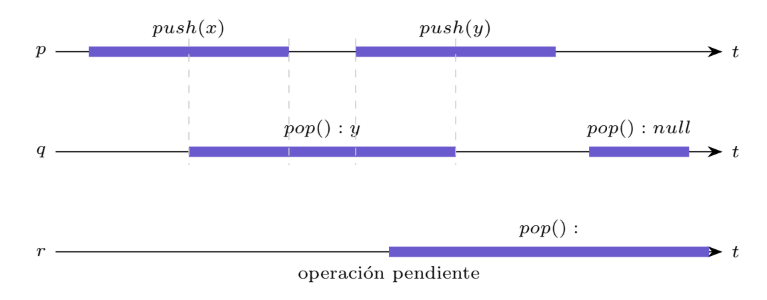
\includegraphics[width=0.8\textwidth]{Imagenes/image-1.png}
    \vspace{-10pt}
\end{figure}
\begin{enumerate}
    \item \textcolor{dkgreen}{¿Es linealizable con respecto a una pila? De ser así, incluye una linearización y especifica la \textit{extension} de $H$ y $complete(H')$.}
\end{enumerate}
Sea $H$ la ejecución (historia concurrente) de la imagen, se quiere saber si $H$ es linealizable \textbf{con respecto a una pila (estructura LIFO)}. La ejecución $H$ es linealizable si existe alguna historia secuencial legal $S$, tal que $S\equiv complete(H)$. Por lo tanto, basta que exhibamos alguna $S$ que cumpla con esto.
\par
Denotaremos que $X$ es concurrente (se traslapa) a $Y$ como $X||Y$, y denotaremos que $X$ precede a (termina antes que) $Y$ como $X<Y$. Recordemos además que:
\begin{itemize}
    \item Todo par de operaciones concurrentes entre sí, se ordenan entre ellas de la forma que más convenga, es decir, $X||Y$ es equivalente a $Y||X$.
    \item Las operaciones precedentes entre sí mantienen su ordenen la transformación, es decir que si $X<_H Y$, entonces $X <_J Y$ (con $J$ transformación de $H$).
\end{itemize}
Primero, descubramos que operaciones o tareas son concurrentes y precedentes entre sí. Las reglas que se cumplen en $H$ son:
\begin{enumerate}[label=\arabic*.]
    \item $push(x) \text{ } || \text{ } pop():y$
    \item $pop():y \text{ } || \text{ }  push(y) \text{ }  || \text{ } pop():$
    \item $pop(): \text{ }  || \text{ } pop():null$
    \item $push(x) < push(y)$
    \item $push(x) < pop():$
    \item $push(x) < pop():null$
    \item $pop():y < pop():null$
    \item $push(y) < pop():null$
\end{enumerate}
Notemos que la historia $H$ tiene una invocación pendiente: la única operación del hilo $r$ ($pop():$) no tiene respuesta. Para transformar $H$ en una historia secuencial $S$, necesitamos encontrar alguna extensión $H'$ tal que $H'=complete(H)$.
\par
Considerando todas las invocaciones completas de $H$, veamos que en algún punto $x$ y $y$ entran en la pila, y en otro punto $y$ salió de la pila, por la regla 6, 7 y 8, para que $pop():null$ solo es posible si $x$ salió de la pila. Afortunadamente, la linealizabilidad nos deja decidir si completamos o borramos las invocaciones pendientes, por lo que elegimos completar la invocación $pop():$ con una respuesta: $pop():x$. Por lo tanto, \textcolor{red}{la extensión $H'=complete(H)$} queda como:
\begin{figure}[H]
    \centering
    \vspace{-10pt}
    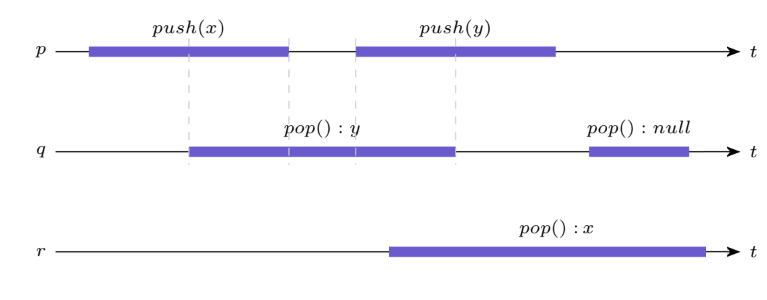
\includegraphics[width=0.8\textwidth]{Imagenes/image-3a.png}
    \vspace{-10pt}
\end{figure}
Completando y reordenando (visualmente) nuestras reglas, tenemos:
\begin{enumerate}[label=\arabic*.]
    \item $push(x) \text{ } || \text{ } pop():y$
    \item $push(y) \text{ } || \text{ }  pop():y \text{ }  || \text{ } pop():x$
    \item $pop():x \text{ }  || \text{ } pop():null$
    \item $push(x) < push(y)$
    \item $push(x) < pop():$
    \item $push(x) < pop():null$
    \item $pop():y < pop():null$
    \item $push(y) < pop():null$
\end{enumerate}
Podemos exhibir la siguiente \textcolor{red}{historia secuencial $S$}:
\begin{equation*}
    S = push(x) <push(y)<pop():y<pop(x)<pop():null
\end{equation*}
\begin{figure}[H]
    \centering
    \vspace{-10pt}
    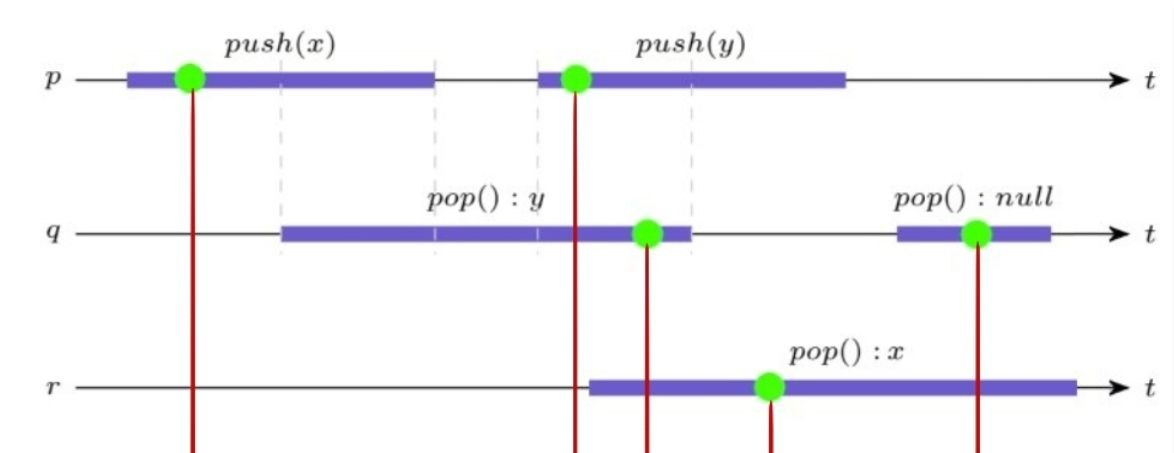
\includegraphics[width=0.8\textwidth]{Imagenes/image-3b.png}
    \vspace{-10pt}
\end{figure}
Como $S$ cumple con todas las 8 reglas de nuestras operaciones en $H'$, entonces existe $S$ una historia secuencial legal tal que $S\equiv complete(H)$.
\par
\textcolor{red}{$\therefore H$ es \textbf{linealizable} con respecto a una pila.}

\item[\textbf{4.}] \textbf{[20 min/20 puntos]} \textcolor{dkgreen}{Una propiedad de corrección se define como \textbf{componible} (o modular) si la validez del sistema global está garantizada siempre que cada uno de sus objetos componentes sea correcto de manera independiente. En computación concurrente, esta característica es vital para el diseño de sistemas modulares: nos permite diseñar y verificar objetos (como una Pila $A$ y una Pila $B$) por separado, con la certeza de que, al integrarlos en un mismo programa, el sistema resultante preservará dicha propiedad.}
\par
\textcolor{dkgreen}{A diferencia de otras condiciones de corrección, la \textit{linealizabilidad} es una propiedad componible. Considera, por ejemplo una ejecución $H$ cuyas proyecciones individuales son linealizables:}
\begin{itemize}
    \item \textcolor{blue}{ $H|A = push(x) \rightarrow pop():x$ }
    \item \textcolor{blue}{ $H|B = push(y) \rightarrow pop():y$ }
\end{itemize}
\textcolor{dkgreen}{Debido a que la linealizabilidad es modular, la historia global $H$ es linealizable si existe una historia secuencial legal S que respete el orden de tiempo real de todas las operaciones. En este caso, la historia $S$ resultante es:}
\begin{equation*}
    \textcolor{blue}{ S=A.push(x) < B.push(y)<B.pop():y<A.pop():x }
\end{equation*}
\begin{figure}[H]
    \centering
    \vspace{-10pt}
    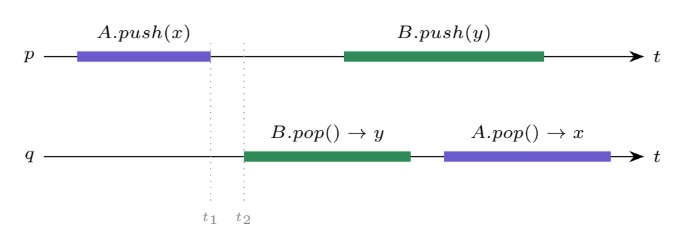
\includegraphics[width=0.8\textwidth]{Imagenes/image-2.png}
    \vspace{-10pt}
\end{figure}
\textcolor{dkgreen}{Considera dos pilas $A$ y $B$. Analiza la siguiente historia $H$:}
\begin{figure}[H]
    \centering
    \vspace{-10pt}
    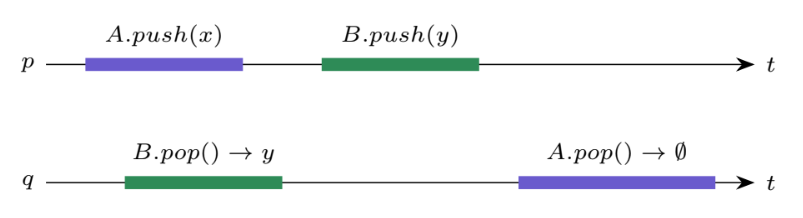
\includegraphics[width=0.8\textwidth]{Imagenes/image-3.png}
    \vspace{-10pt}
\end{figure}
\begin{enumerate}
    \item \textcolor{dkgreen}{¿Es $H|A$ secuencialmente consistente? (Pista: Busca un orden global).}
\end{enumerate}
Para la subhistoria $H|A$, solo consideramos la proyección sobre la pila $A$, es decir, la operación $A.push(x)$ del hilo $p$, y la operación $A.pop()\rightarrow\emptyset$ del hilo $q$. Dado que la consistencia secuencial permite reordenar operaciones de distintos hilos siempre y cuando se respete el orden local, al ser únicas las operaciones en cada hilo (para $H|A$), podemos construir la historia secuencial $S_A = A.pop()\rightarrow \emptyset < A.push(x)$. Claramente esta secuencia es legal porque si la extracción ocurre antes de la inserción de $x$ (asumiendo una pila vacía al inicio), es correcto devolver $\emptyset$.\\
Por lo tanto, \textcolor{red}{$H|A$ si es secuencialmente consistente}.
\begin{enumerate}
    \setcounter{enumi}{2}
    \item \textcolor{dkgreen}{¿Es $H|B$ secuencialmente consistente? }
\end{enumerate}
Nuevamente solo consideramos las operaciones sobre la pila $B$: la operación $B.push(y)$ del hilo $p$, y la operación $B.pop()\rightarrow y$ del hilo $q$.
Al tratarse de operaciones únicas en su respectivo hilo (se mantiene el orden local), se construye la siguiente historia secuencial (por consistencia secuencial): $S_B=B.push(y)<B.pop()\rightarrow y$.\\
Es claro que es una secuencia legal respecto a una pila, por lo tanto \textcolor{red}{$H|B$ si es secuencialmente consistente}.
\begin{enumerate}
    \setcounter{enumi}{3}
    \item \textcolor{dkgreen}{¿Es la historia global $H$ secuencialmente consistente?}
\end{enumerate}
Para que $H$ sea secuencialmente consistente únicamente debe respetar el orden local de cada hilo:
\begin{enumerate}[label=\arabic*.]
    \item $A.push(x) <B.push(y) \quad$ (orden estricto por el hilo $p$)
    \item $B.pop()\rightarrow y <A.pop()\rightarrow \emptyset \quad $ (orden estricto por el hilo $q$)
\end{enumerate}
Tratemos de construir paso a paso una historia legal:
\begin{itemize}
    \item Tomamos a la regla 2 del hilo $q$ como base:\\
    $S=B.pop()\rightarrow y <A.pop()\rightarrow \emptyset$
    \item Para que la pila $B$ haya extraído al elemento $y$, debió meterlo antes. Agregamos entonces la operación $B.push(y)$ del hilo $p$ al inicio. Al tratarse de hilos separados, por consistencia secuencial podemos insertar esta nueva operación donde convenga:
    $S=B.push(y) <B.pop()\rightarrow y <A.pop()\rightarrow \emptyset$
    \item Por la misma consistencia secuencial, al realizar el paso anterior, esto nos obliga a añadir la operación $A.push(x)$ antes de $B.push(y)$ para poder cumplir con el orden obligatorio legal del hilo $p$:\\
    $S=A.push(x)<B.push(y) <B.pop()\rightarrow y <A.pop()\rightarrow \emptyset$
    \item Sin embargo a pesar que esta es una secuencia legal de $S$ (cumple las reglas de orden local), no es una ejecución correcta respecto a pilas: La pila $B$ se mantiene correcta porque primero mete a $y$ y luego lo saca; pero en la pila $A$ se nos dice que mete a $x$ pero cuando se intenta sacar el elemento, $A.pop$ devuelve vacío. Esto es incorrecto.
\end{itemize}
La situación no cambia si tomamos como base la regla 1 para intentar construir una secuencia legal y correcta $S$.
Por lo tanto, \textcolor{red}{$H$ no es secuencialmente consistente}.\\
Más aún, encontramos un ejemplo donde a pesar de que las proyecciones individuales son secuencialmente consistentes, la integración final (historia global) no necesariamente es secuencialmente consistente. Por lo tanto, \textcolor{red}{la consistencia secuencial no es componible}.

\item[\textbf{5.}] \textbf{[15 min/10 puntos]} \textcolor{dkgreen}{En una píla asíncrona, el hilo $p$ termina su operación y el sistema entra en un periodo de ``inactividad''.}
\begin{figure}[H]
    \centering
    \vspace{-10pt}
    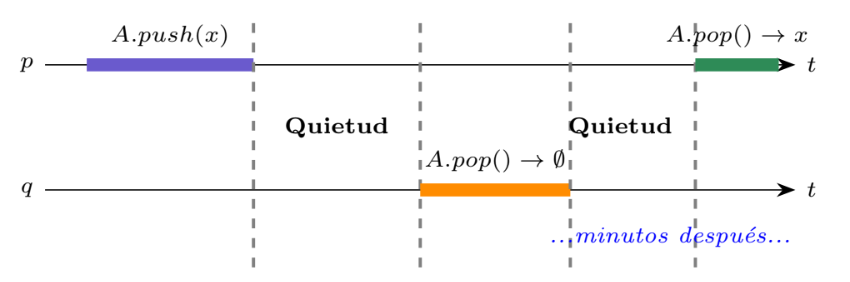
\includegraphics[width=0.8\textwidth]{Imagenes/image-4.png}
    \vspace{-10pt}
\end{figure}
\begin{enumerate}
    \item \textcolor{dkgreen}{¿Por qué esta ejecución cumple con Consistencia Eventual pero rompe la Consistencia en la Inactividad?}

    Esta ejecución cumple con \textbf{Consistencia Eventual} porque esta propiedad permite que se observen resultados atrasados, siempre y cuando eventualmente el sistema converja al estado correcto. Esto se cumple cuando $p$ realiza el $pop()$ y recibe $x$, ya que finalmente el sistema termina reflejando el estado final esperado.
    
    Por otro lado, no se cumple la \textbf{Consistencia en la Inactividad} porque entre el $push(x)$ y el $pop()$ de $q$ hubo un periodo de quietud. Por lo tanto, el $push(x)$ tuvo que haber quedado completamente antes del $pop()$ de $q$. En consecuencia, cuando $q$ realizó el $pop()$, la pila ya debía contener a $x$ y el resultado correcto era recibir $x$, pero recibió $null$. Como el periodo de quietud impide reordenar el $push(x)$ para colocarlo después del $pop()$, la ejecución no puede corresponder a un orden secuencial válido y se rompe la Consistencia en la Inactividad.
\end{enumerate}



\item[\textbf{6.}] \textbf{[20 min/25 puntos]} \textcolor{dkgreen}{Considera la siguiente clase $Visibility$:}\\
\par
\begin{lstlisting}[numbers=none,language=Java,caption=Clase "VisibilityField"]
class Visibility {
    Shared Variables:
\end{lstlisting}

\begin{lstlisting}[
    firstnumber=1,
    numbers=left,
    language=Java
]
    int x=0;
    volatile Boolean flag=false;
    void writerThread() {
        try {
            Thread.sleep(1000);
            x = 1;
            flag = true;
        } catch(InterruptedException e) {}
    }
    void readerThread() {
        while(!flag){}
        int y = 100/x;
    }
\end{lstlisting}

\begin{enumerate}
    \item \textcolor{dkgreen}{¿Es posible que el método \texttt{readerThread()} divida entre cero? Argumenta porqué.}

    No, en este caso no es posible dividir entre 0. Esto se debe a que \texttt{flag} es \texttt{volatile}. El hilo que escribe primero cambia \texttt{x} a 1 y después cambia \texttt{flag} a \texttt{true}. Cuando el sistema observa que la bandera ya está en \texttt{true}, también puede observar el cambio anterior de \texttt{x}, por lo que \texttt{x} ya vale 1 y no puede realizarse una división entre cero.

    
    \item \textcolor{dkgreen}{Si ambas variables son \texttt{volatile}, ¿es posible que el método \texttt{readerThread()} divida entre cero? Argumenta porqué.}

    No, en este caso tampoco es posible, aunque ambas sean volatile al igual que en la respuesta anterior primero se cambiaría el valor de x a 1 y ya después flag a true, por lo que de igual forma no se puede dividir entre 0. 

    \item \textcolor{dkgreen}{Si ninguna de las dos variables es \texttt{volatile}, ¿es posible que el método \texttt{readerThread()} divida entre cero? Argumenta porqué.}

    Para este caso si es posible que se pueda dividir entre 0, como ya ninguna variable es volatile el sistema puede pasar la bandera a true antes de poner x=1 porque ya se trata de dos instrucciones independientes, es decir, el sistema ve la bandera levantada o en true y sale del ciclo, al salir puede encontrar x=0, así que en este caso si se puede dividir entre 0. Igual otro caso que podemos encontrar es que los valores estén desactualizados, por lo que al llegar a la división puede que x se encuentre con el valor de 0. 

\end{enumerate}
\end{enumerate}

\end{document}

